\documentclass[]{article}

\usepackage{multirow,hhline,graphicx,array}
\usepackage{makecell}
\usepackage{geometry}
\usepackage{pdfpages}
\usepackage{titlesec}
\usepackage{float}
\usepackage{ulem}
\usepackage{caption2}
\usepackage[hidelinks]{hyperref}

\makeatletter
\def\@maketitle{%       
	\newpage
	\null
	\vskip 14em%
	\begin{center}%
		\let \footnote \thanks
		{\LARGE \@title \par}%
		\vskip 12em%
		{\large
			\lineskip .5em%
			\begin{tabular}[t]{c}%
				\@author
			\end{tabular}\par}%
		\vskip 1em%
		{\large \@date}%
	\end{center}%
	\par
	\vskip 1.5em}
\makeatother
%opening
\title{\Huge COP5725 - Database Management Systems\vspace{2.8em} \LARGE \textbf{Project Deliverable 3:} Weather Recording System}
\author{
	\Large Group 19:\qquad He,Jiahui,\\
	\Large \qquad\qquad\qquad\qquad Shi,Qinxuan,\\
	\Large \qquad\qquad\qquad\qquad Wang,Shihuan,\\
	\Large \qquad\qquad\qquad\qquad\qquad Zhang,Guanglong
}
\date{}
\special{papersize=8.5in,11in}
\geometry{left=2.5cm,right=2.5cm,top=1.5cm,bottom=1.5cm}


\begin{document}
	
	\maketitle
	\clearpage
	
	\tableofcontents
	\clearpage
	
	\section{Quality of the transformation of the ER diagram into a collection of relation schemas.}
	
	\subsection{Improved ER Diagram}
	
	\begin{figure}[H]
		\centering
		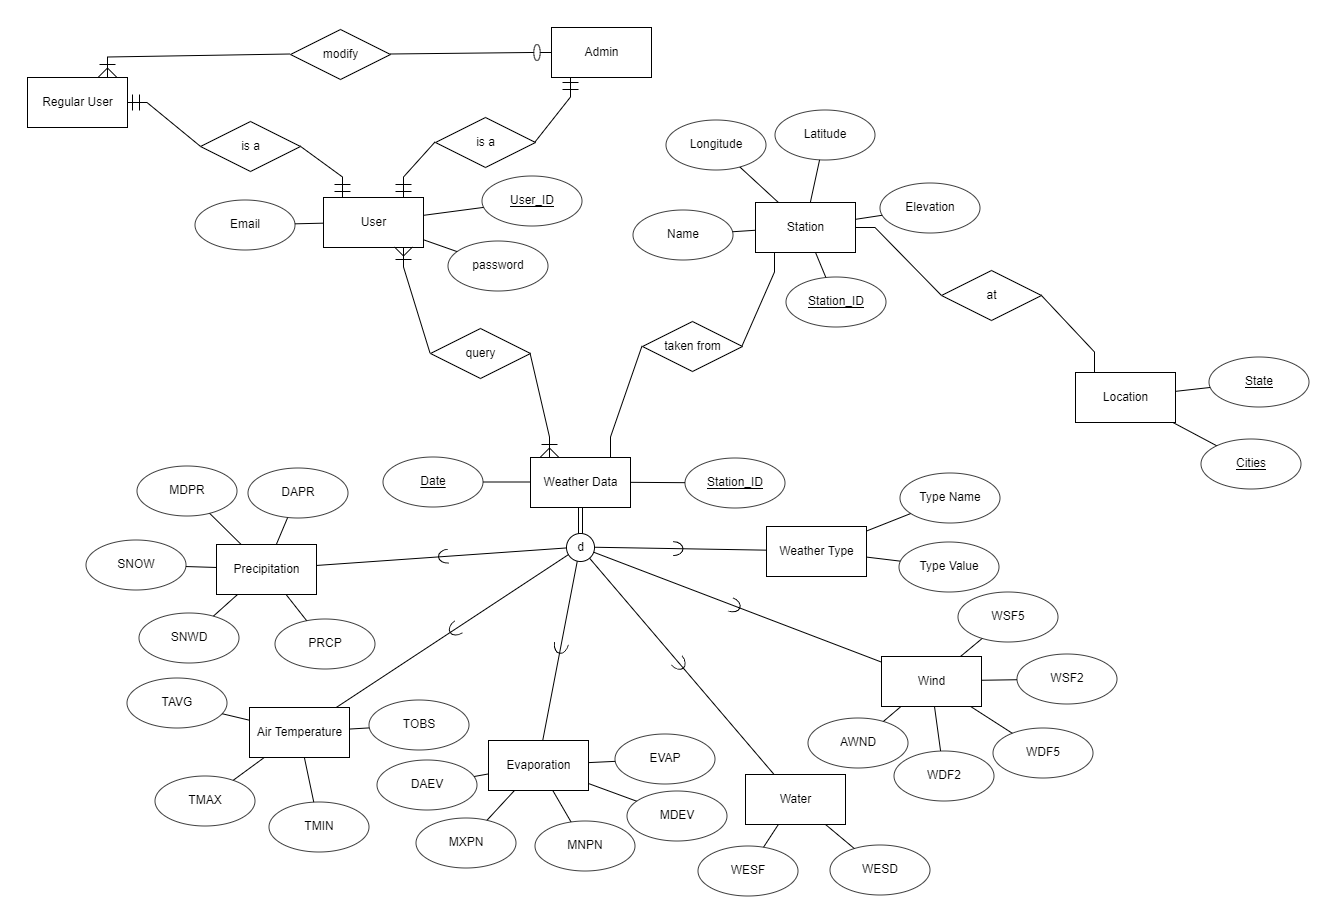
\includegraphics[width=1\linewidth]{../d3-p/ER}
		\caption{ER Diagram}
		\label{fig:er}
	\end{figure}
	
	\subsection{Relational Schema}
	
	\noindent User(\uline{User\_{ID}: Integer}, Email: String, password: String) \\
	
	\noindent We know from the ER diagram that the 'User' entity acts as a superclass, and it has three attributes. The first attribute is the unique attribute 'User\_ID', the domain of this attribute is Integer. The second attribute is 'password', the domain of this attribute is String. The third attribute is 'Email', the domain of this attribute is String.  \\
	
	\noindent Regular\_User(\uline{User\_{ID}: Integer}) \\
	
	\noindent Admin(\uline{User\_{ID}: Integer}) \\
	
	\noindent The subclasses of the superclass 'User' have two entities, they are disjoint from each other. One is the 'Regular\_User' entity, with the unique attribute 'User\_ID', the domain of this attribute is String. The other is the 'Admin' entity, with the unique attribute 'User\_ID', the domain of this attribute is String.    \\
	
	\noindent Station(\uline{Station\_ID: String}, Name: String, Latitude: Float, Longitude: Float, Elevation: Float)  \\
	
	\noindent All the weather data is taken from the physical stations. The relation of ‘Station’ has attributes of (Station\_ID: String, Name: String, Latitude: Float, Longitude: Float, Elevation: Float). The primary key is Station\_ID. The data type of Station\_ID is strings that contain characters and numbers with lengths no longer than 10. Name\_ contains characters only. Latitudes and Longitudes are numbers with a maximum length of 13 and the maximum number of decimal is 10. The positive and negative values of these two values indicate their directions(North, South, East, and West). Elevation’s values are ranged from 0 to 999 with one decimal place.  \\
	
	\noindent Location(\uline{State: String}, \uline{City: String})  \\
	
	\noindent When users query a set of weather data of a certain location, they input City and State. The data type of State and City is String with a length no longer than 20.   \\
	
	\noindent WeatherData(\uline{Station\_ID: String}, \uline{Data\_Time: Date})   \\
	
	\noindent As the ER diagram shows, ‘WeatherData’ is the superclass of all subclasses(e.g. AirTemperature, Water). Its two attributes are also primary keys(Station\_ID: String, Data\_Time: Date). The data type of Station\_ID is a unique string that contains characters and numbers with lengths no longer than 10. Date contains data type of Date.    \\
	
	\noindent Precipitation(\uline{Station\_ID: String}, \uline{Data\_Time: Date}, DAPR: Float, MDPR: Float, SNOW: Float, SNWD: Float, PRCP: Float)\\
	
	\noindent According to the ER diagram, ‘Precipitation’ is a subclass of its super class ‘WeatherData’. Just like the ‘WeatherData’, ‘Precipitation’ also has two attributes, ‘Station\_ID’ and ‘Data\_Time’, which form a pair to become the primary key of this relationship. Learnt from the data file and its explanation document, ‘DAPR’ is short for Number of days included in the multiday precipitation total, ‘MDPR’ is short for Multiday precipitation total, ‘PRCP’ means precipitation, ‘SNWD’ stands for snow depth and ‘SNOW’ refers to snowfall. All these attributes are measured in inches and the data type is float.  \\
	
	\noindent AirTemperature(\uline{Station\_ID: String}, \uline{Data\_Time: Date}, TAVG: Integer, TMAX: Integer, TMIN: Integer, TOBS: Integer)\\
	
	\noindent Also as a subclass of ‘WeatherData’, ‘AirTemperature’ has a pair of primary keys (Station\_ID, Data\_Time) and its own attributes. ‘TAVG’ means the average temperature, ‘TMAX’ means the maximum temperature, ‘TMIN’ refers to the minimum temperature and ‘TOBS’ represents temperature at the time of observation. We choose Fahrenheit as the unit of measurement, and the data types of these attributes are all integers.   \\
	
	\noindent Evaporation(\uline{Station\_ID: String}, \uline{Data\_Time: Date}, DAEV: Integer, MXPN: Float, MNPN: Float, MDEV: Float, EVAP: Float)\\
	
	\noindent As an important member of weather information, ‘Evaporation’ is also a subclass of ‘Weather’, like other subclasses, it uses the pair (Station\_ID, Data\_Time) as its primary keys. In addition, ‘DAEV’ refers to the number of days included in the multiday evaporation total, ‘MXPN’ is short for daily maximum temperature of water in an evaporation pan, ‘MNPN’ is daily minimum temperature of water in an evaporation pan, ‘MDEV’ means multiday evaporation total and ‘EVAP’ means evaporation of water from evaporation pan. The data type of ‘DAEV’ should be integer and the data types of the other attributes are floats.   \\
	
	\noindent Water(\uline{Station\_ID: String}, \uline{Data\_Time: Date}, WESF: Float, WESD: Float)\\
	
	\noindent We can learn from the ER Diagram that the relation 'Water' is a subclass of the super class 'WeatherData'. Since Generalizations are not represented by an own relation, the key of 'WeatherData' (\uline{Station\_ID: String}, \uline{Data\_Time: Date}) is also be used as the key of 'Water'. Besides, 'Water' has two other attributes. 'WESF' means the water equivalent of snowfall, which domain is Integer, and 'WESD' means the water equivalent of snow on the ground, which domain is also Integer. \\
	
	\noindent Wind(\uline{Station\_ID: String}, \uline{Data\_Time: Date}, WSF5: Float, WSF2: Float, WDF5: Integer, WDF2: Integer, AWND: Float)\\
	
	\noindent The relation of 'Wind' is also the subclass of 'WeatherData'. So, the key is (\uline{Station\_ID: String}, \uline{Data\_Time: Date}). There are several other attributes. 'WSF5' means fatest 5-second wind speed, the domain of this attribute is Float. 'WSF2' means fatest 2-minute wind speed, the domain of this attribute is Float. 'WDF5' means the direction of fatest 5-second wind speed, the domain of this attribute is Float. 'WDF2' means the direction of fatest 2-minute wind speed, the domain of this attribute is Float. 'AWMD' means average wind speed, the domain of this attribute is Float.  \\
	
	\noindent WeatherType(\uline{Station\_ID: String}, \uline{Data\_Time: Date}, TypeName: Integer, TypeValue: Boolean)\\
	
	\noindent The relation of 'WeatherType' is also the subclass of 'WeatherData'. So, the key is (\uline{Station\_ID: String}, \uline{Data\_Time: Date}). There are two other attributes. 'TypeName' is the type of the Weather, since the set of data uses number like '01', '02' to represent the weather Type, we decide to define the domain as Integer. 'TypeValue' is exactly a boolean value, it means whether or not the weather belongs to the type.  \\
	
	\clearpage
	
	\section{Quality of the transformation of the collection of relation schemas into a collection of SQL table schemas.}
	
	\noindent According to the relational schema, the 'User' entity has three attributes. The user registers for an account by using Email and Password. We define them as VARCHAR2(20). Since ‘User\_ID’ is a number string automatically generated by the system, we define this as Integer.  \\
	
	\noindent According to the relational schema, ‘Regular\_User’ has one attribute. We define them as Integer which is the same as ‘User’ table.   \\
	
	\noindent According to the relational schema, ‘Admin’ has one attribute. We define them as Integer which is the same as ‘User’ table.  \\
	
	\begin{figure}[H]
		\centering
		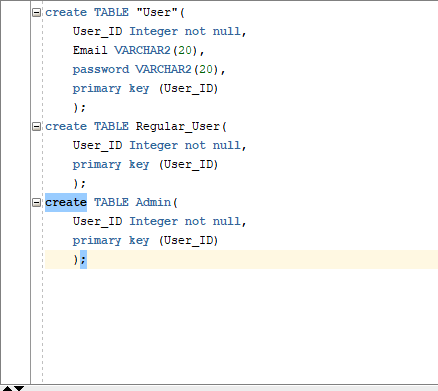
\includegraphics[width=0.8\linewidth, height=0.35\textheight]{../d3-p/part1}
		\caption{}
		\label{fig:part1}
	\end{figure}
	
	\begin{figure}[H]
		\centering
		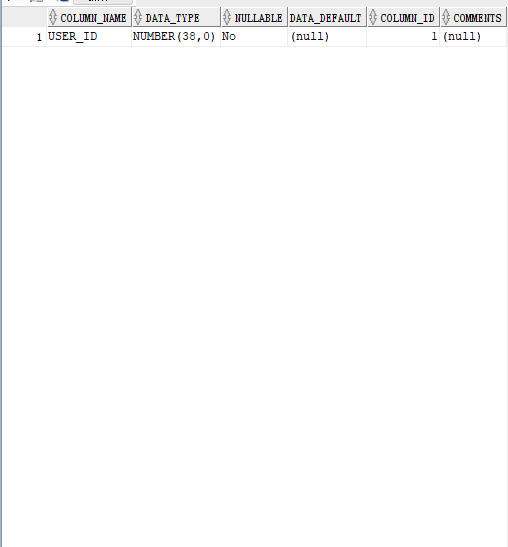
\includegraphics[width=0.8\linewidth, height=0.3\textheight]{../d3-p/part1-1}
		\caption{}
		\label{fig:part1-1}
	\end{figure}
	
	\begin{figure}[H]
		\centering
		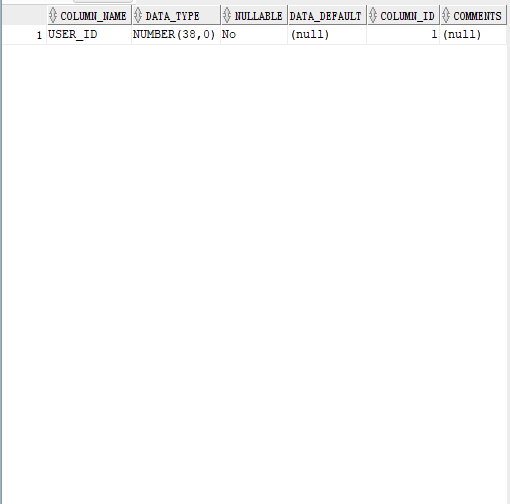
\includegraphics[width=0.8\linewidth, height=0.3\textheight]{../d3-p/part1-2}
		\caption{}
		\label{fig:part1-2}
	\end{figure}

	\begin{figure}[H]
		\centering
		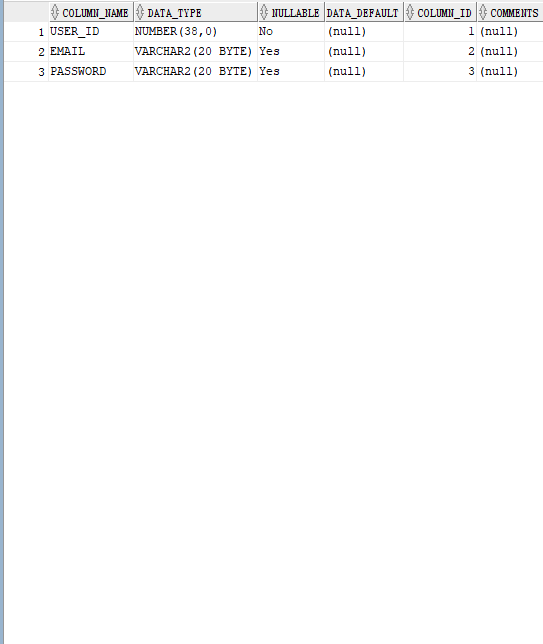
\includegraphics[width=0.8\linewidth, height=0.3\textheight]{../d3-p/part1-3}
		\caption{}
		\label{fig:part1-3}
	\end{figure}

	\noindent All the weather data is taken from the physical stations. The relation of ‘Station’ has attributes of (Station\_ID: String, Name: String, Latitude: Float, Longitude: Float, Elevation: Float). The primary key is Station\_ID. The data type of Station\_ID is strings that contain characters and numbers with lengths no longer than 10. Name\_ contains characters only. Latitudes and Longitudes are numbers with a maximum length of 13 and the maximum number of decimal is 10. The positive and negative values of these two values indicate their directions(North, South, East, and West). Elevation’s values are ranged from 0 to 999 with one decimal place.    \\
	
	\noindent When users query a set of weather data of a certain location, they input City and State. The data type of State and City is String with a length no longer than 20.   \\
	
	\noindent As the ER diagram shows, ‘WeatherData’ is the superclass of all subclasses(e.g. AirTemperature, Water). Its two attributes are also primary keys(Station\_ID: String, Data\_Time: Date). The data type of Station\_ID is a unique string that contains characters and numbers with lengths no longer than 10. Date contains data type of Date.    \\

	\begin{figure}[H]
		\centering
		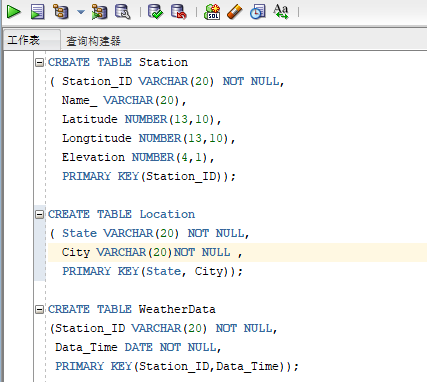
\includegraphics[width=0.7\linewidth, height=0.4\textheight]{../d3-p/part2}
		\caption{}
		\label{fig:part2}
	\end{figure}
	
	\begin{figure}[H]
		\centering
		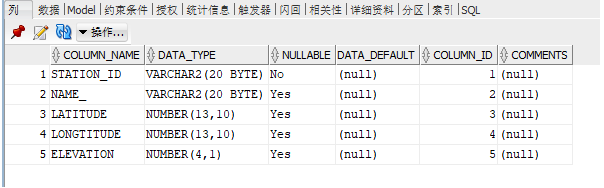
\includegraphics[width=0.7\linewidth]{../d3-p/part2-1}
		\caption{}
		\label{fig:part2-1}
	\end{figure}
	
	\begin{figure}[H]
		\centering
		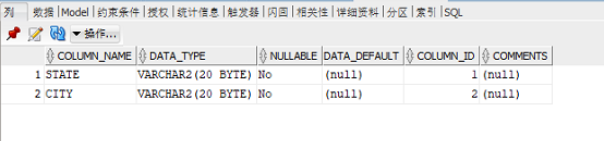
\includegraphics[width=0.7\linewidth]{../d3-p/part2-2}
		\caption{}
		\label{fig:part2-2}
	\end{figure}
	
	\begin{figure}[H]
		\centering
		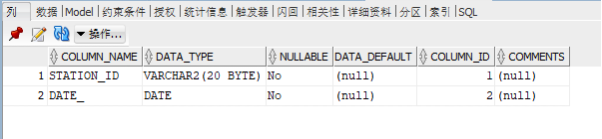
\includegraphics[width=0.7\linewidth]{../d3-p/part2-3}
		\caption{}
		\label{fig:part2-3}
	\end{figure}
	

	\noindent According to the relation schema and the dataset, except ‘Station\_ID’ and ‘Data\_Time’, which should be the same as in the ‘WeatherData’ table, the other attributes in the table ‘Precipitation’ are reserved for two decimal places, and the integer part is set to three digits. Combined with the data type of the oracle database, numeric(5, 2) is selected as the data type.  \\
	
	\noindent In this table, attributes ‘Station\_ID’ and ‘Data\_Time’ should be the same as in the ‘WeatherData’ table since ‘AirTemperature’ is a subclass of ‘WeatherData’. Besides, the data type of all other attributes should be integer as we do have this data type in oracle database.   \\
	
	\noindent Like other subclasses, attributes ‘Station\_ID’ and ‘Data\_Time’ should be the same as in the ‘WeatherData’. In addition, we use integer for ‘DAEV’ since the count of days must be an integer. The other attributes in the table ‘Evaporation’ are reserved for two decimal places, and the integer part is set to three digits. Taking the data type of the oracle database into consideration, numeric(5, 2) is selected as the data type.  \\

	\begin{figure}[H]
		\centering
		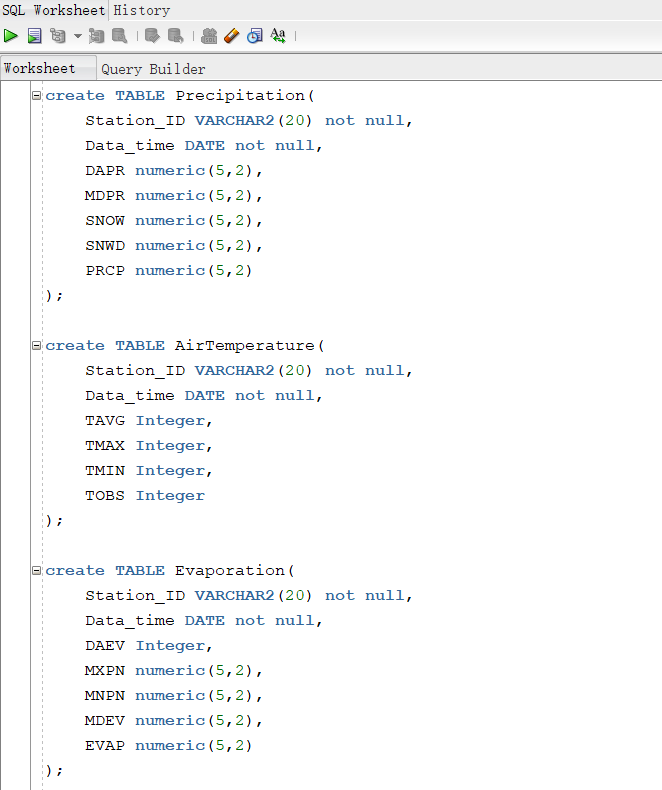
\includegraphics[width=0.7\linewidth, height=0.33\textheight]{../d3-p/part3}
		\caption{}
		\label{fig:part3}
	\end{figure}
	
	\begin{figure}[H]
		\centering
		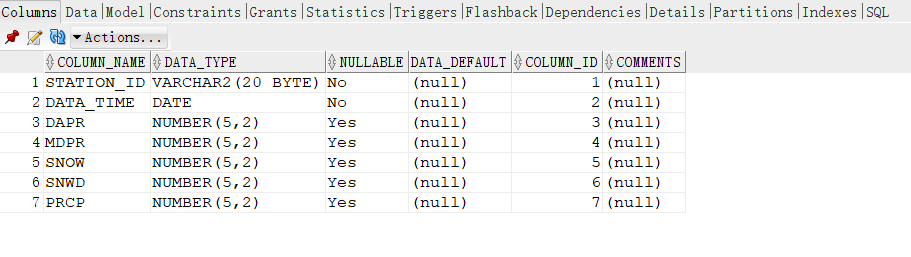
\includegraphics[width=0.8\linewidth]{../d3-p/part3-1}
		\caption{}
		\label{fig:part3-1}
	\end{figure}
	
	\begin{figure}[H]
		\centering
		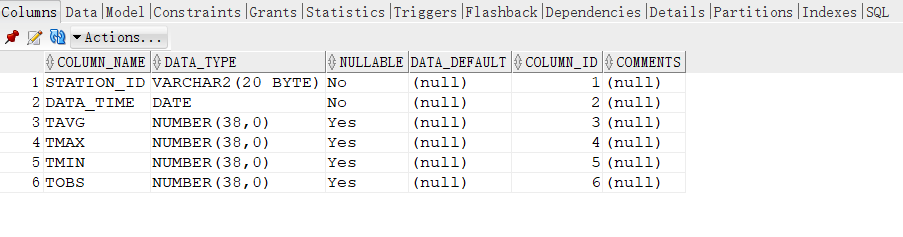
\includegraphics[width=0.8\linewidth]{../d3-p/part3-2}
		\caption{}
		\label{fig:part3-2}
	\end{figure}

	\begin{figure}[H]
		\centering
		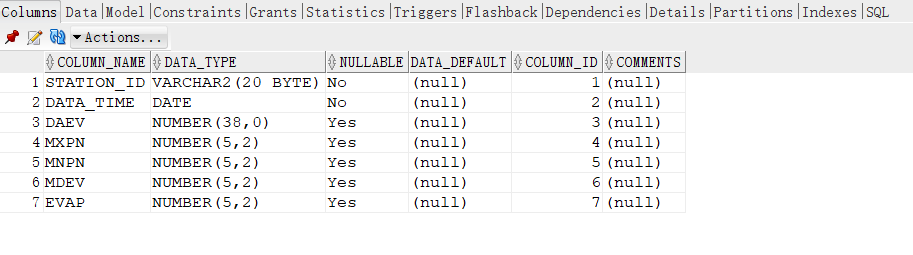
\includegraphics[width=0.8\linewidth]{../d3-p/part3-3}
		\caption{}
		\label{fig:part3-3}
	\end{figure}
	
	\noindent According to the relational schema, the primary key is (Station\_ID, Data\_Time), which is the same as Weather Data table, so I do not describe this again. Since both of the attributes 'WESF' and 'WESD' are required two decimals and the integer part will not exceed three digits, we define them as numeric(5, 2). \\
	
	\begin{figure}[H]
		\centering
		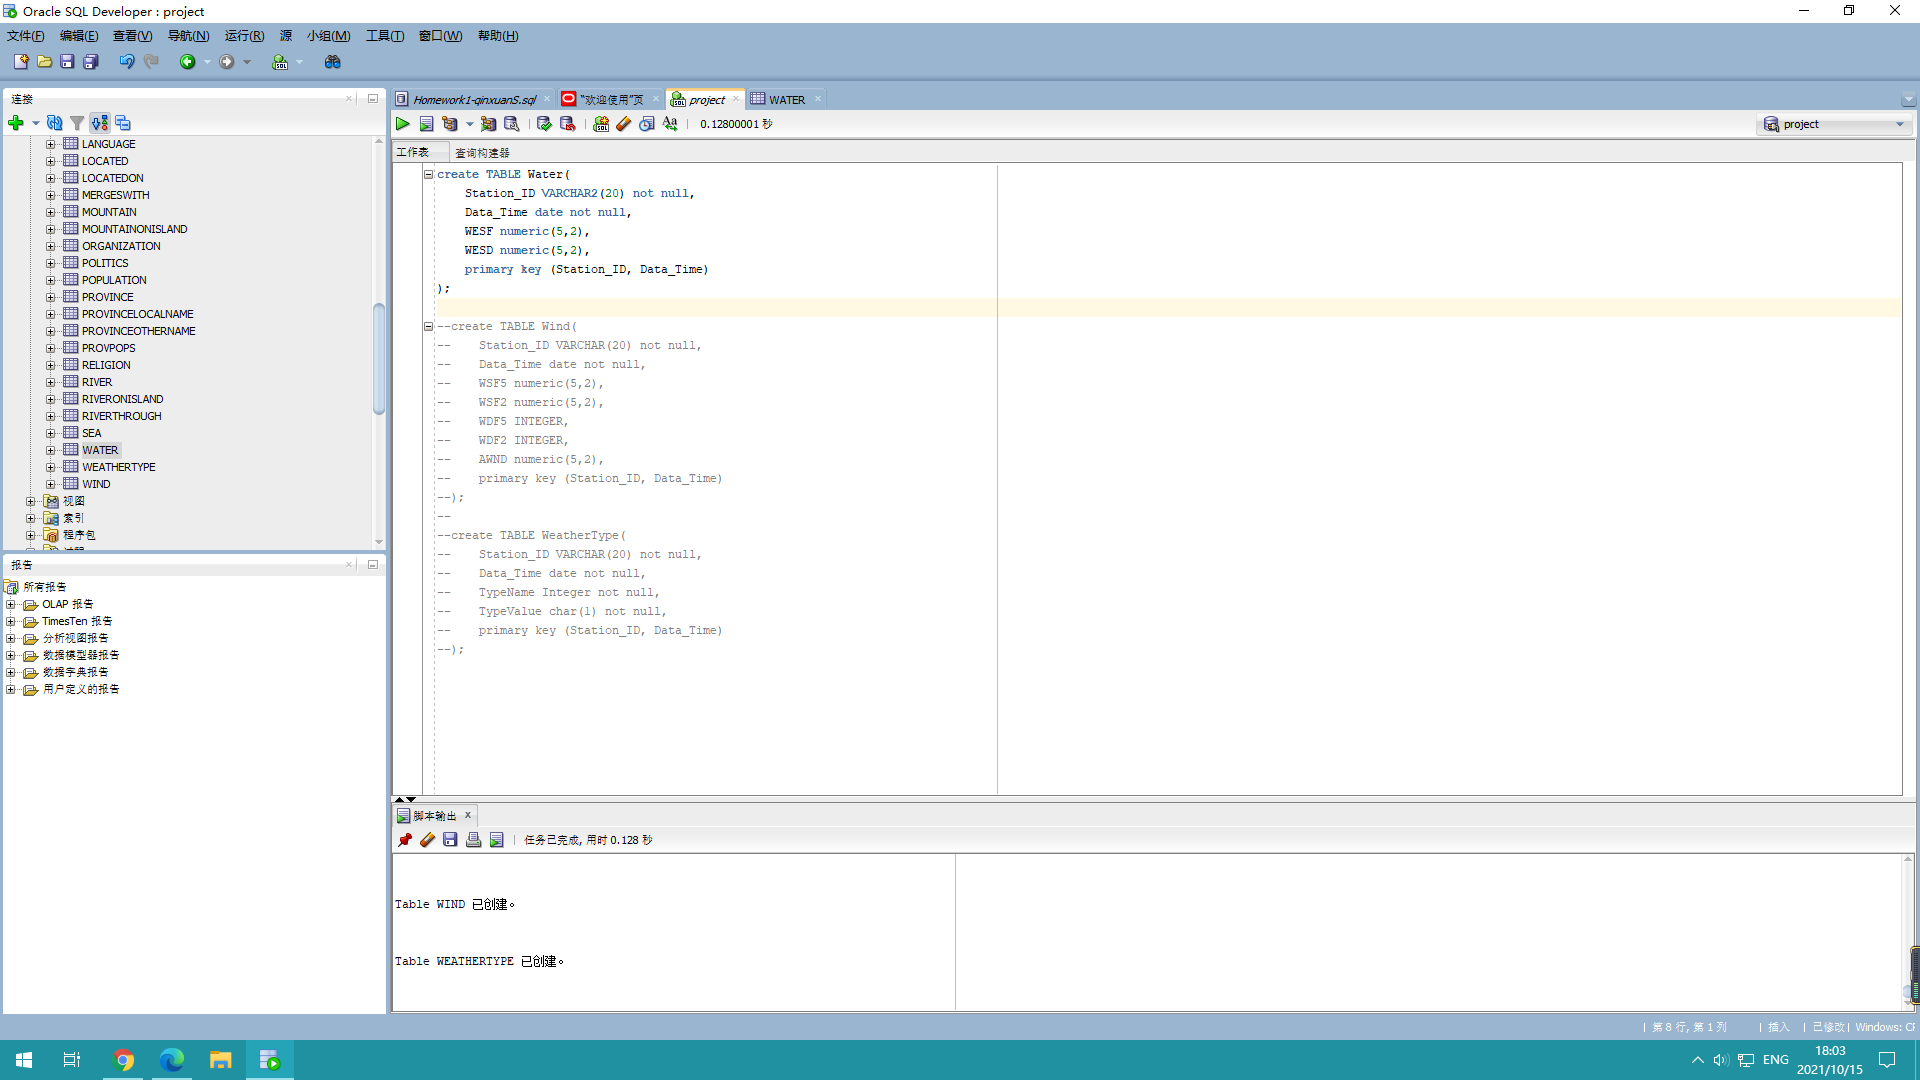
\includegraphics[width=0.95\linewidth]{../d3-p/water-sql}
		\caption{Water-SQL}
		\label{fig:water-sql}
	\end{figure}

	\noindent Here is the snapshot of the Table of Water. \\
	\begin{figure}[H]
		\centering
		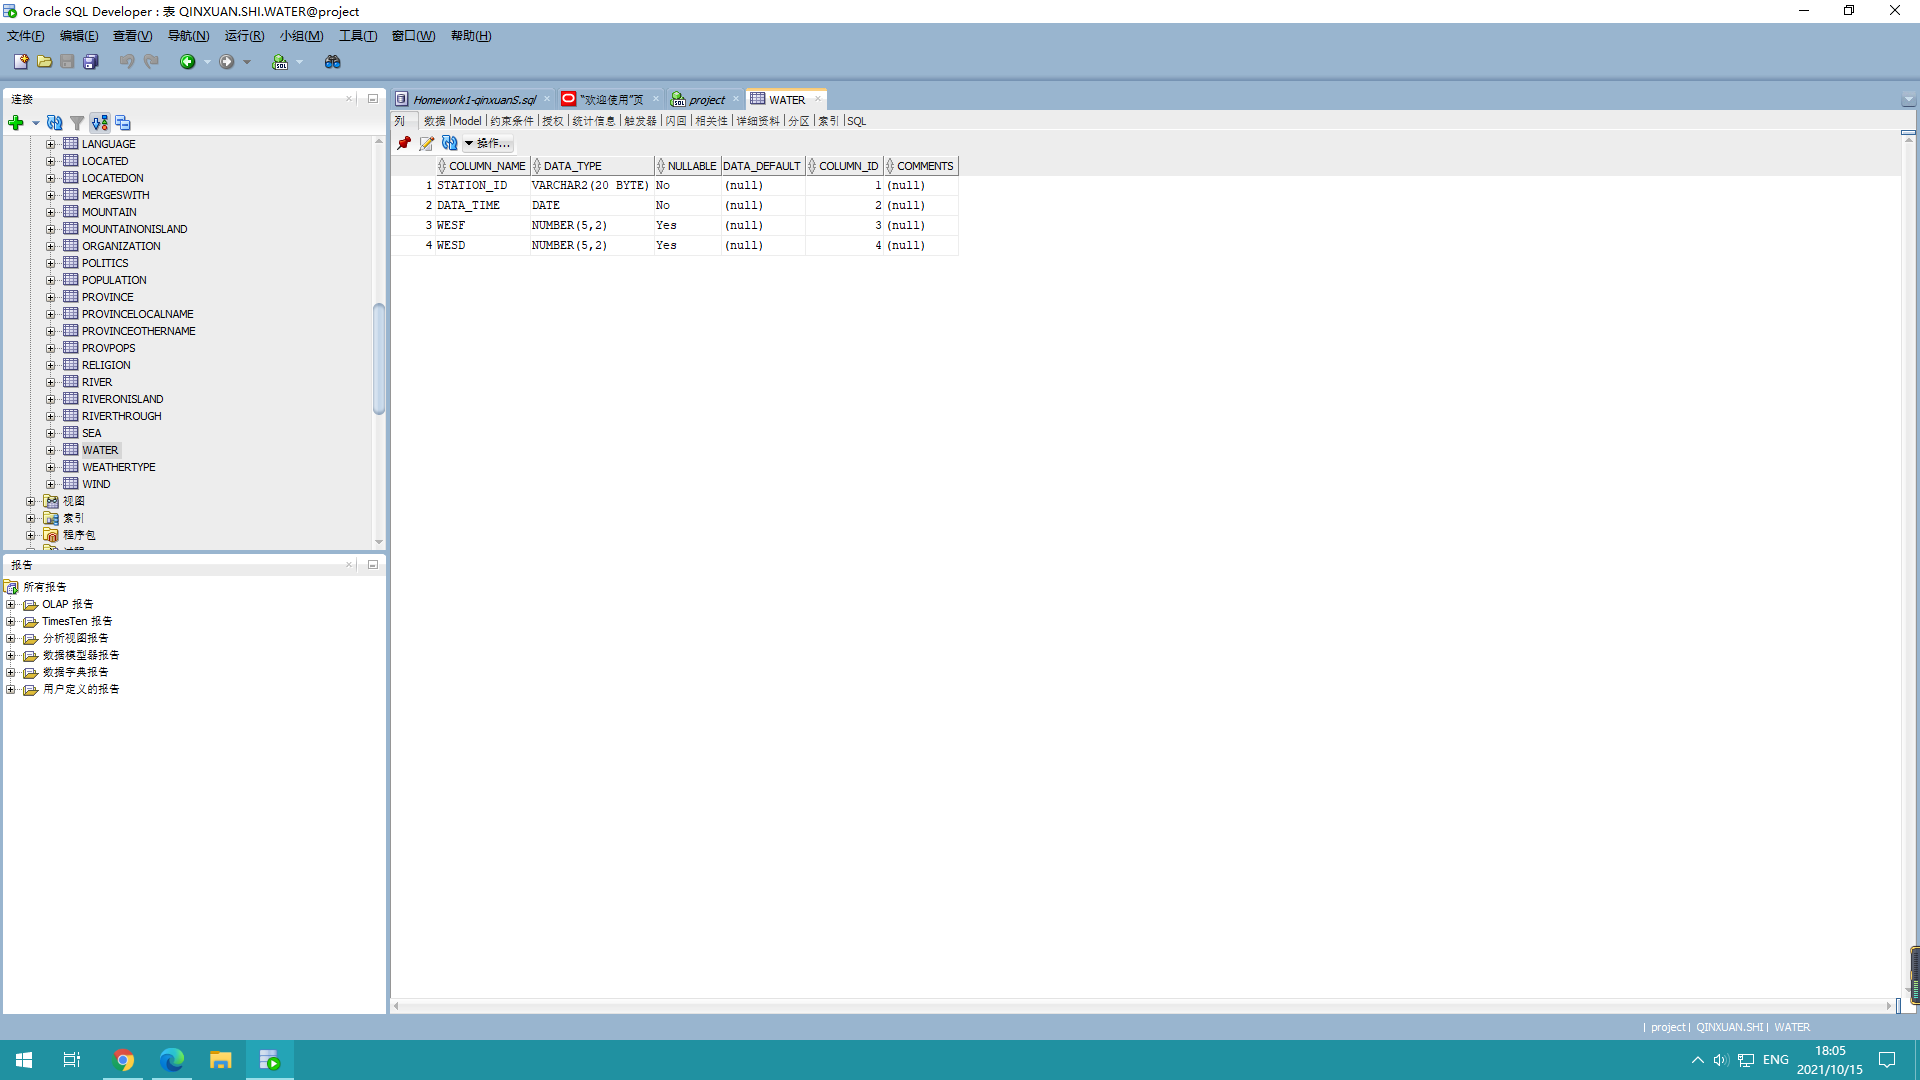
\includegraphics[width=0.95\linewidth]{../d3-p/water}
		\caption{Water-Table}
		\label{fig:water}
	\end{figure}
	
	\noindent According to the relational schema, the primary key is also (Station\_ID, Data\_Time), which is the same as Weather Data table. Since the attributes 'WSF5', 'WSF2' and 'AWND' are required two decimals and the integer part will not exceed three digits, we define them as numeric(5, 2). Besides, the attributes 'WDF5' and 'WDF2' are using Integer to represent wind speed, so we define them to be Integer.\\
	
	\begin{figure}[H]
		\centering
		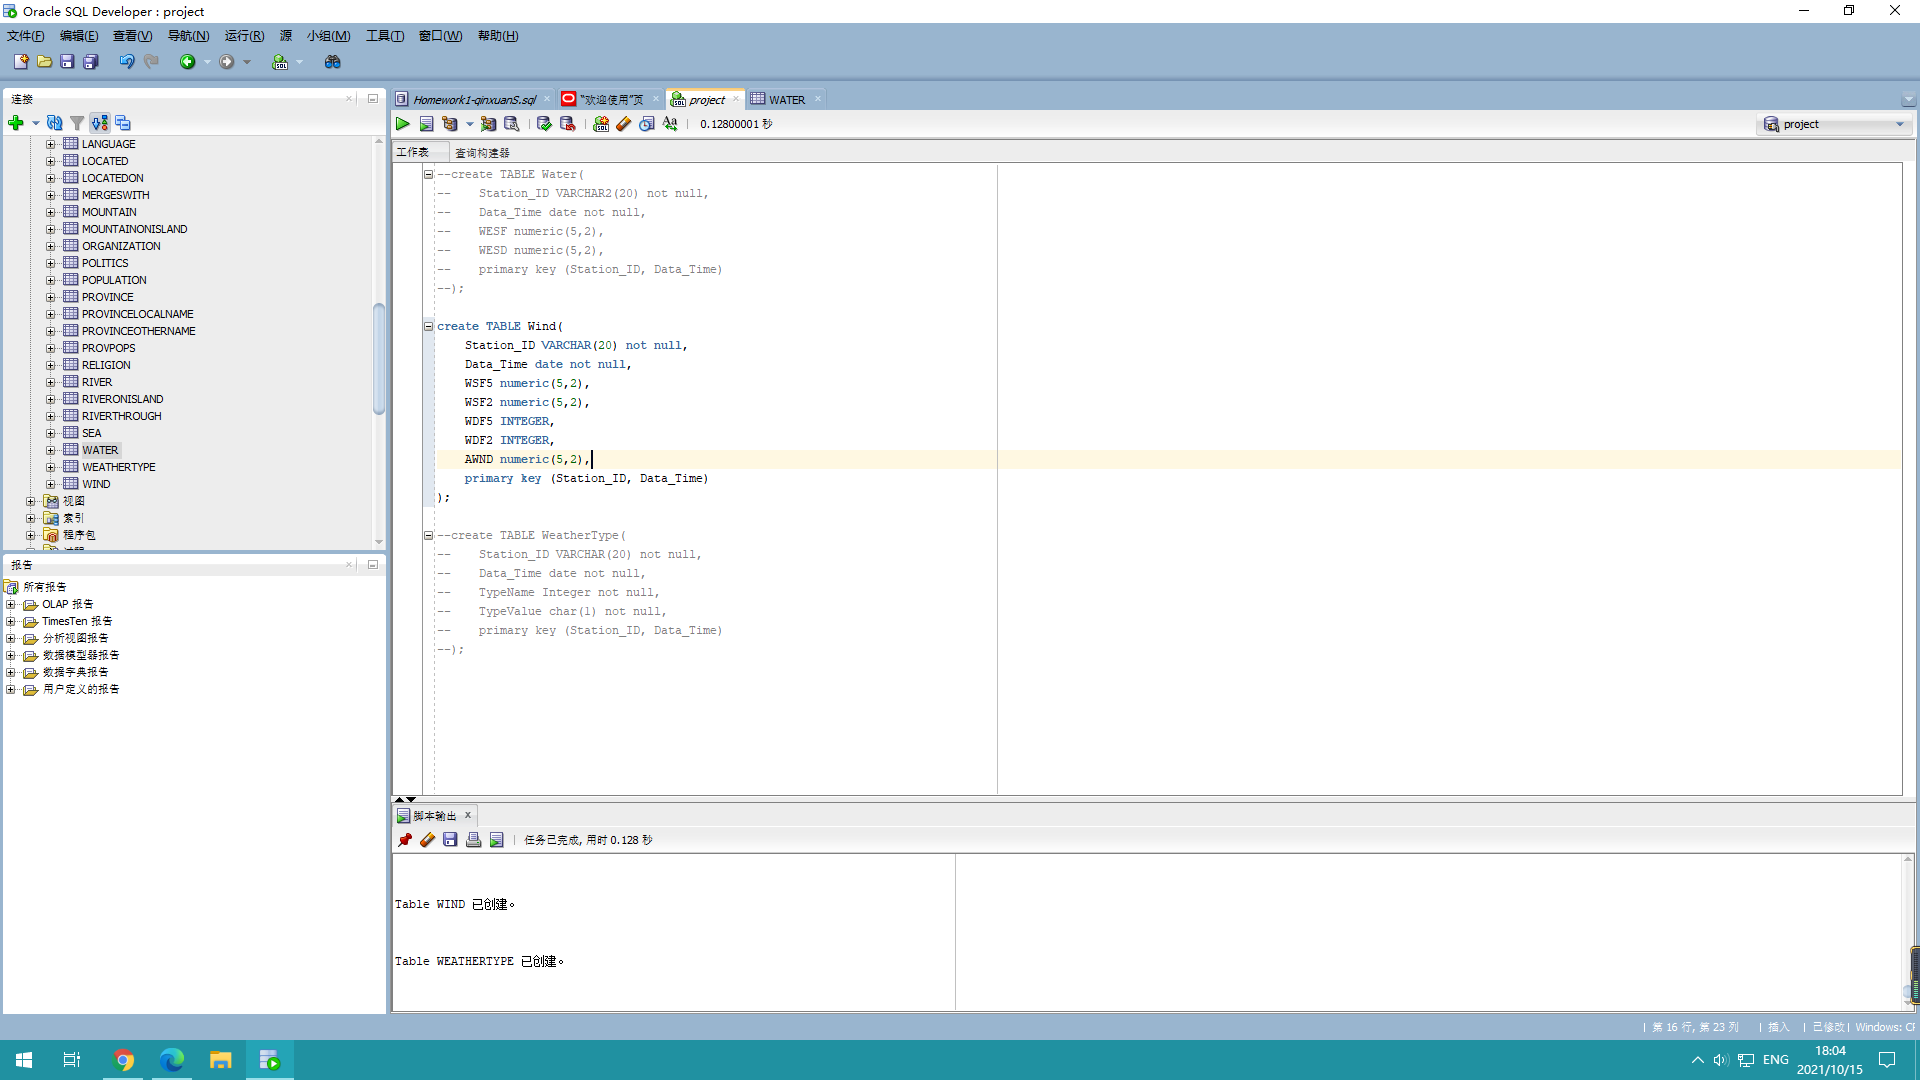
\includegraphics[width=1\linewidth]{../d3-p/wind-sql}
		\caption{Wind-SQL}
		\label{fig:wind-sql}
	\end{figure}
	
	\noindent Here is the snapshot of the Table of Wind. \\
	
	\begin{figure}[H]
		\centering
		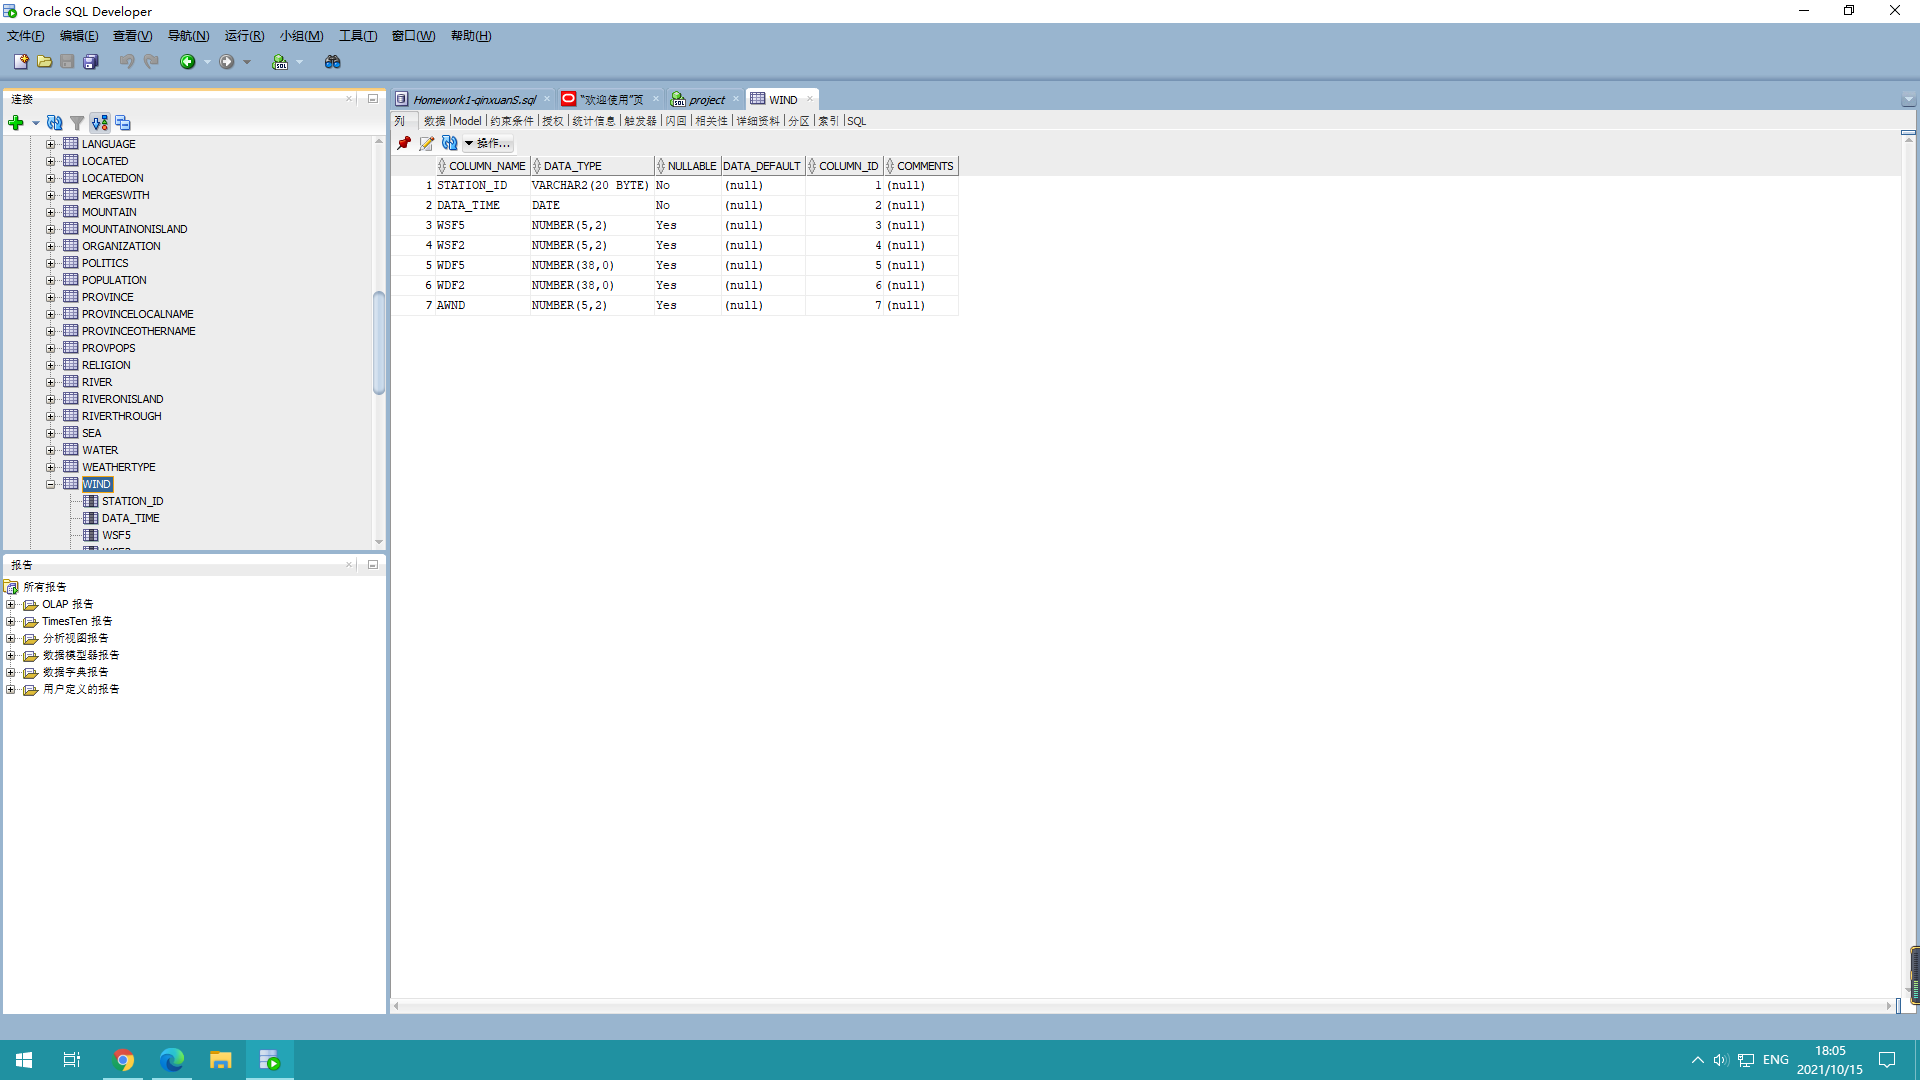
\includegraphics[width=1\linewidth]{../d3-p/wind}
		\caption{Wind-Table}
		\label{fig:wind}
	\end{figure}

	\noindent According to the relational schema, the primary key is (Station\_ID, Data\_Time), which is the same as Weather Data table. Since data sets use format like '01', '02' to represent different weather Type, we define 'TypeName' to be Integer. The 'TypeValue' is exactly a boolean value, which only contains two possible results 'true' or 'false'. However, the Oracle database does not support boolean type, we choose char(1) to represent this boolean value. '0' means false and '1' means true.  \\
	
	\begin{figure}[H]
		\centering
		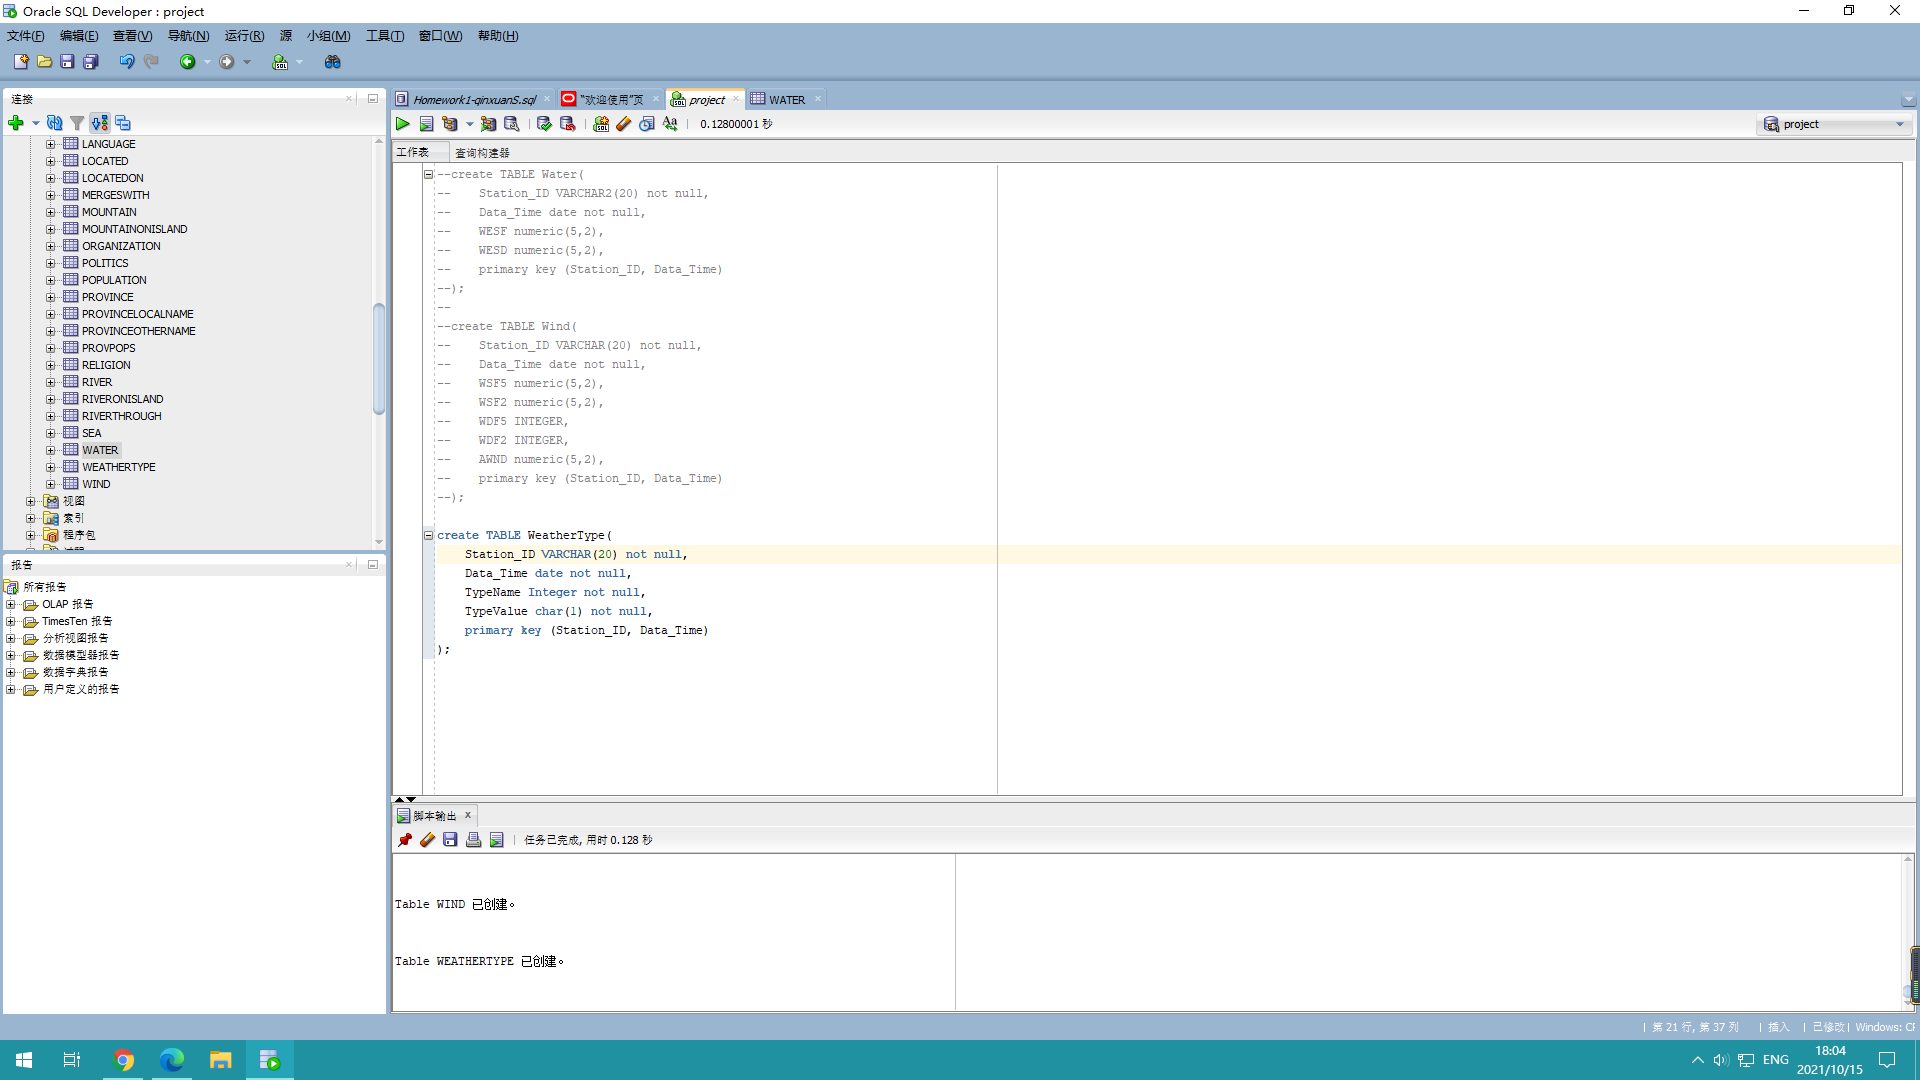
\includegraphics[width=1\linewidth]{../d3-p/weatherType-sql}
		\caption{WeatherType-SQL}
		\label{fig:weathertype-sql}
	\end{figure}

	\noindent Here is the snapshot of the Table of WeatherType. \\

	\begin{figure}[H]
		\centering
		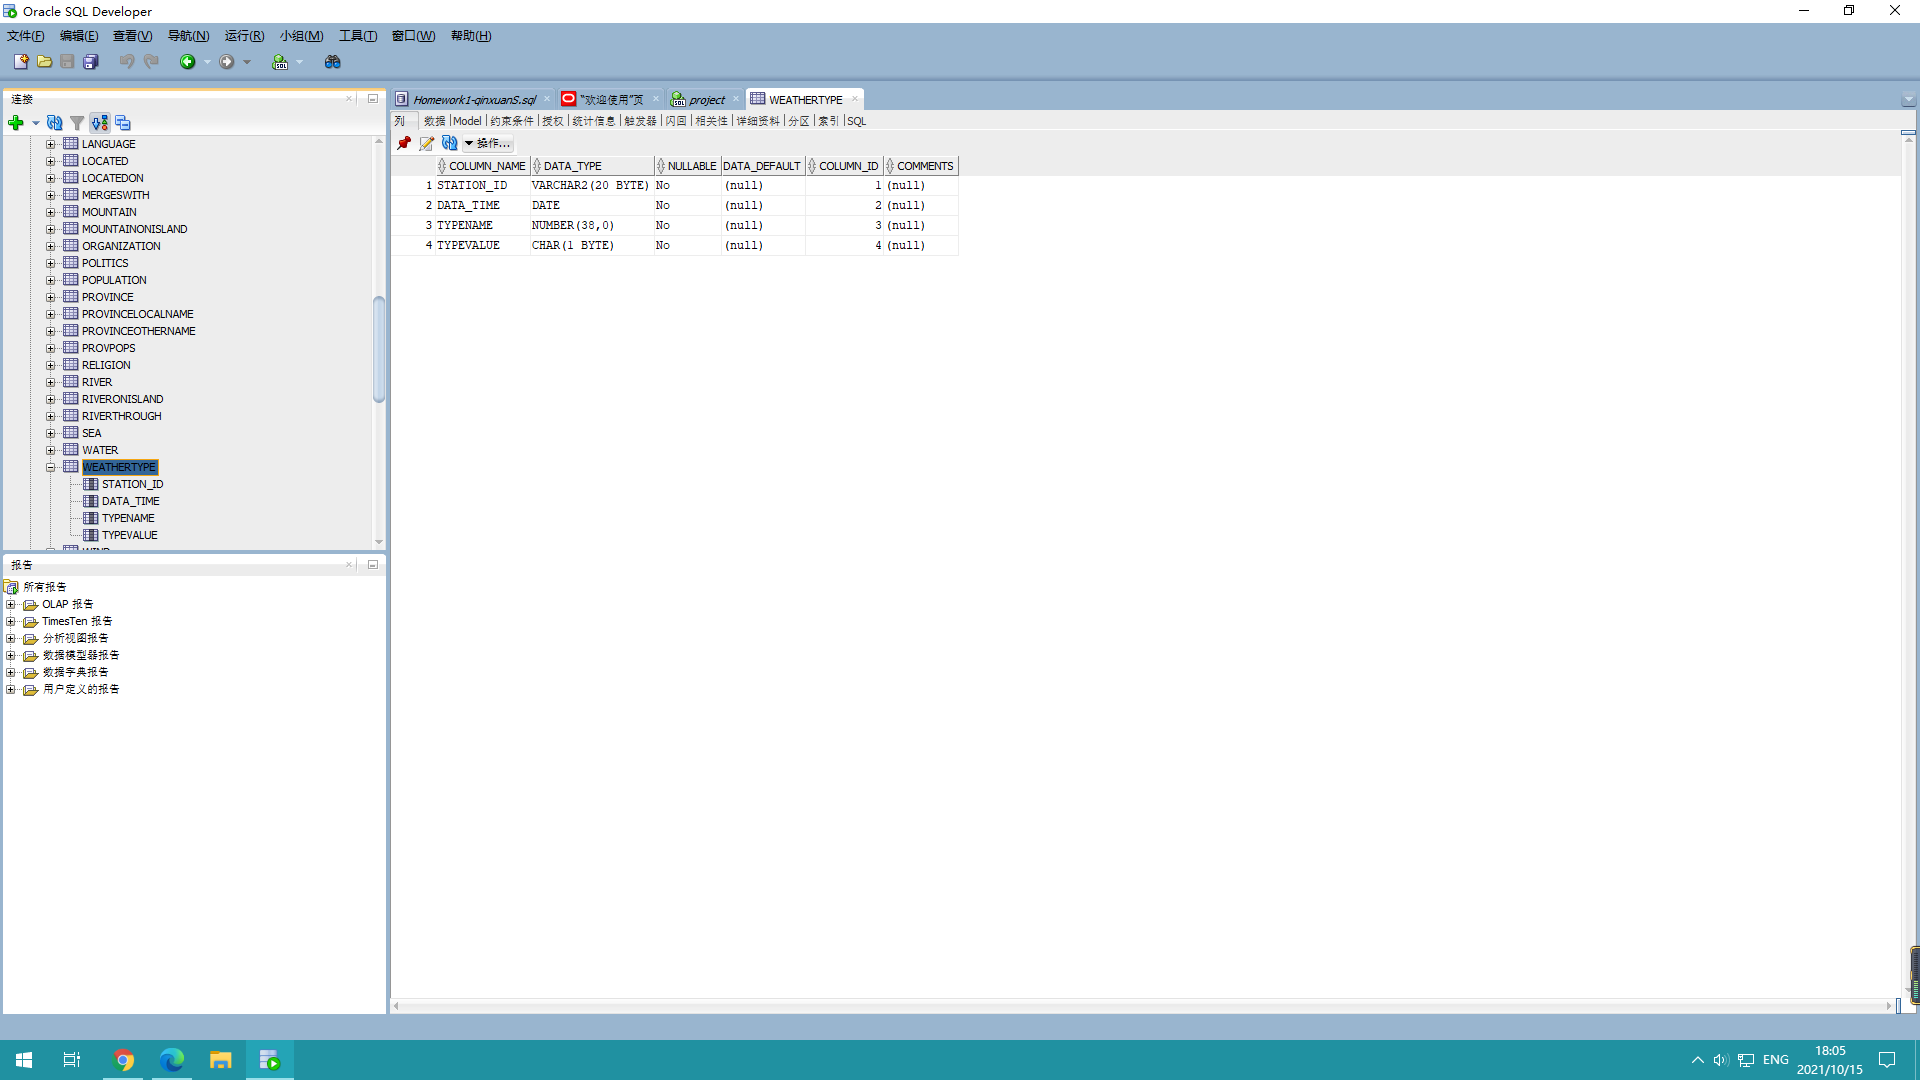
\includegraphics[width=1\linewidth]{../d3-p/weatherType}
		\caption{WeatherType-Table}
		\label{fig:weathertype}
	\end{figure}
	
	
\end{document}
